\newpage

\section{Simulation Analysis}
\label{sec:simulation}
\captionsetup[table]{skip=10pt}

\subsection{Operating Point Analysis for $t<0$}

\vspace{5mm}
\par For $t<0$, $v_s(t)=V_s$ and the system behaves as explained in \ref{teo:2.1}. 

\vspace{3mm}
\par The simulated operating point results (obtained from Ngspice) for the circuit under analysis, which for $t<0$ behaves as explained in subsection \ref{teo:2.1}, are shown in Table \ref{tab_1}. Once again, the positive and negative terminals of the components (and, accordingly, the current directions) were defined as seen on Figure \ref{fig:rc}.

\vspace{3mm}
\par Compared to the theoretical analysis results, one notices a few differences.
\vspace{3mm}
\par Focusing on the obtained nodal voltage levels, an almost exact resemblance is shown, except for the fact that Octave's used result precision is of 7 significant digits (excluding the minus sign), whereas Ngspice always presents 7 significant digits, but counting the minus sign. Even though the numerical roundings of the values present some diminute differences, they are mostly correct. It's worth noting that node 4 (introduced exclusively on the simulation analysis) was created so a zero valued voltage source (working as an ammeter) could be placed in series with resistor 6, allowing the algorithm to measure the current between GND and 7. The same issue takes place with the current values.

\vspace{3mm}
\par Other than that, we could say there's a perfect match on the results obtained from both analysis methods.
\vspace{5mm}

\subsection{Operating Point Analysis for $v_s=0$ and $V_x$ as a replacement for the capacitor}
\label{op_2}

\vspace{5mm}
\par Considering $v_s(t)=0$ (short-circuit) and replacing the capacitor with a voltage source $V_x = V(6)-V(8)$ (where V(6) and V(8) are the voltages in nodes $6$ and $8$ obtained in the previous subsection), we obtain the results on Table \ref{tab_2} (subsection \ref{teo:2.2}). 


\vspace{3mm}
\par The same considerations can be made for the comparison between the theoretical/simulation results, for both voltages and currents, and so one obtains the same value for $R_{eq}$ as shown on table \ref{tab_2}.

\vspace{3mm}
\par The reason behing this type of analysis has been described before. Once again, the values obtained for $V(6)$ and $V(8)$ will be used to describe the initial conditions ($t=0$) for the voltage levels on the capacitor terminals.
\vspace{5mm}

\subsection{Transient analysis - natural solution}

\vspace{5mm}
\par Using the boundary conditions $V(6)$ and $V(8)$ as obtained in \ref{op_2} and \textit{Ngpice}’s transient analysis mode, the natural response of the circuit was simulated (setting $v_s(t)=0$ - short-circuit). Figure\ref{trans} represents the plot for $v_{6n}(t)$ in the interval $[0, 20]$ $ms$. One can easily compare it to the Octave's plot and certify that they are equivalent.

 \begin{figure}[h]
     \centering
         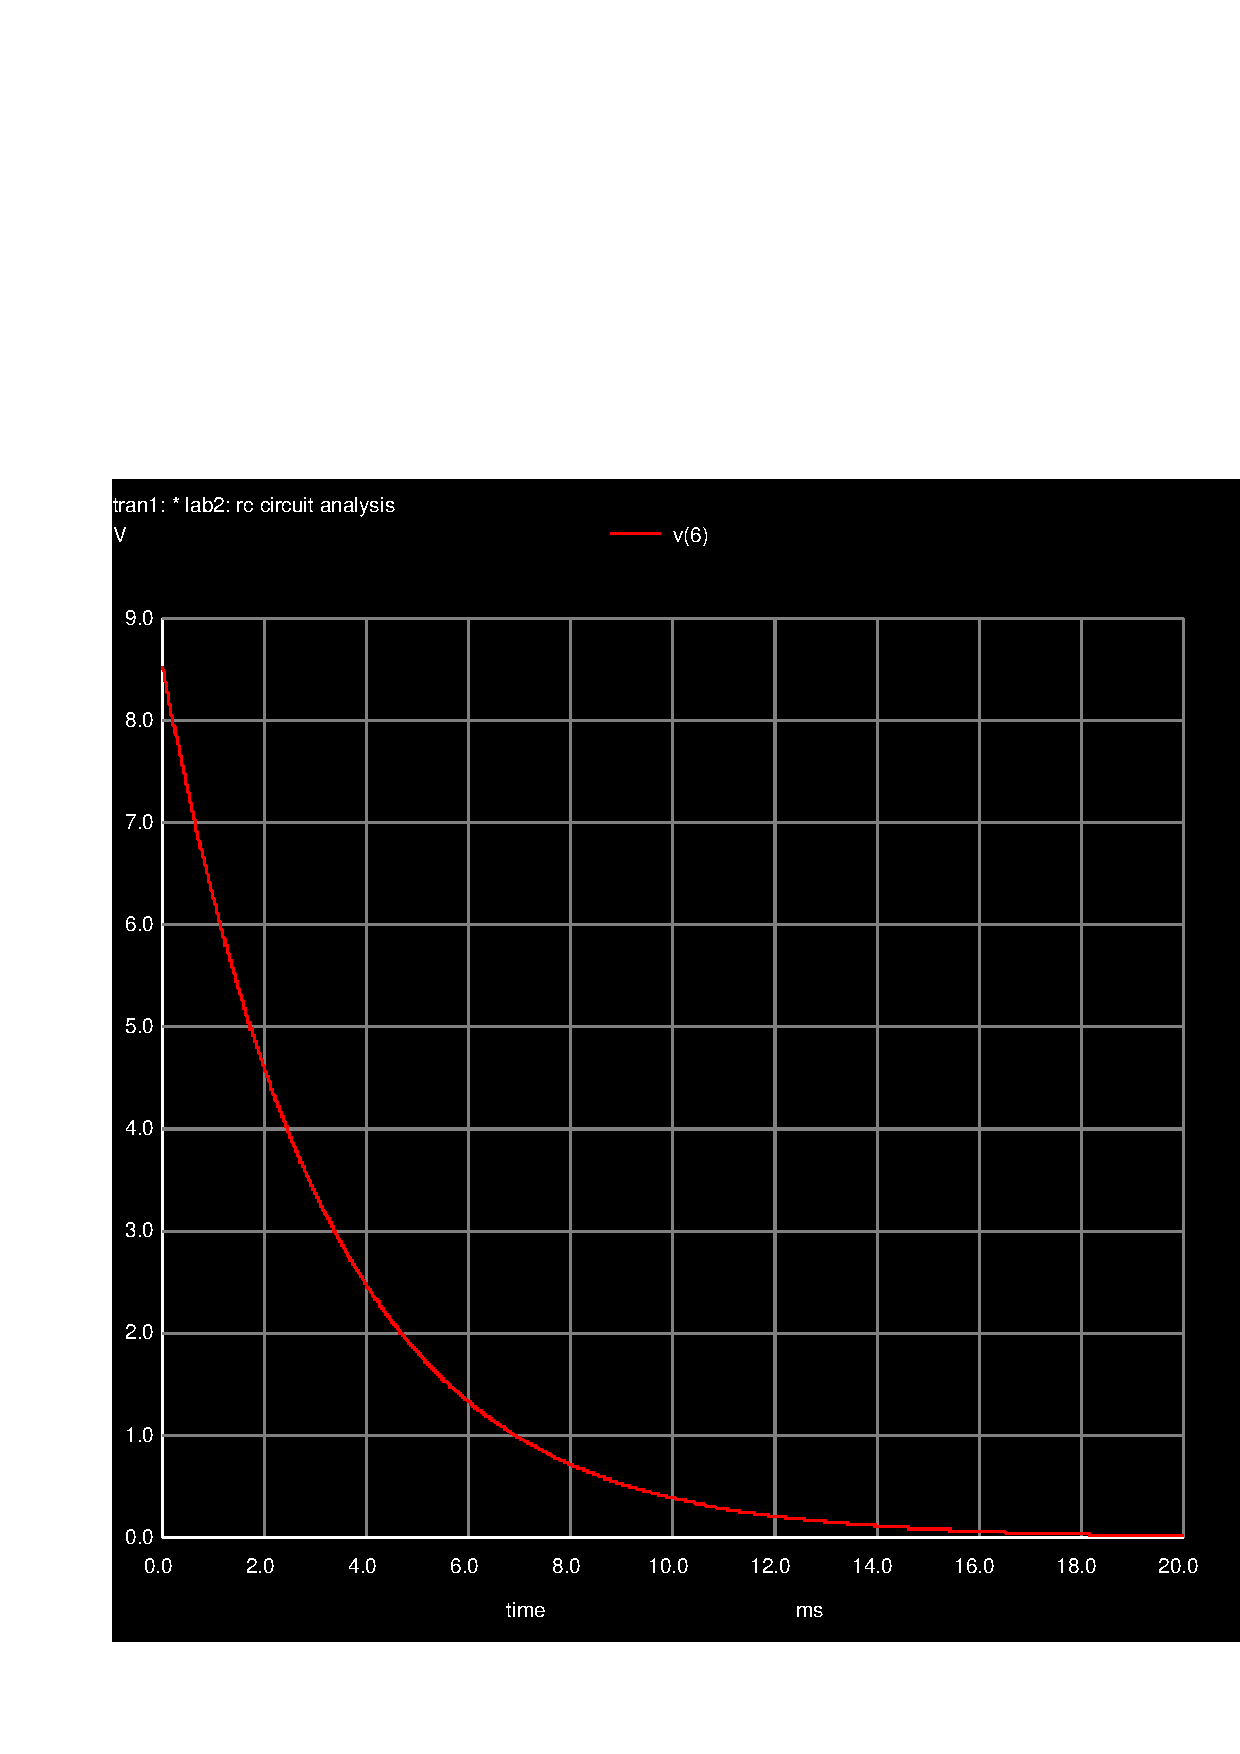
\includegraphics[scale = 0.55]{trans.pdf}
         \caption{$v_{6n}(t)$ in the interval $[0, 20]$ $ms$.}
     \label{trans}
 \end{figure}
 \vspace{5mm}

\subsection{Transient analysis - total solution}

\vspace{5mm}
By reproducing the previous step with $v_s(t)=\sin(2\pi ft)$ ($f=1kHz$), the total response of the circuit (natural + forced solution) was simulated. Figure \ref{total} represents the plot for both $v_s(t)=v_1(t)$ (stimulus) and $v_6(t)$ (response) in the interval $[0, 20]$ $ms$. Once again, we can be certain that Figures \ref{v6t} and \ref{total} represent the same voltage behaviour through time.

 \begin{figure}[h]
     \centering
         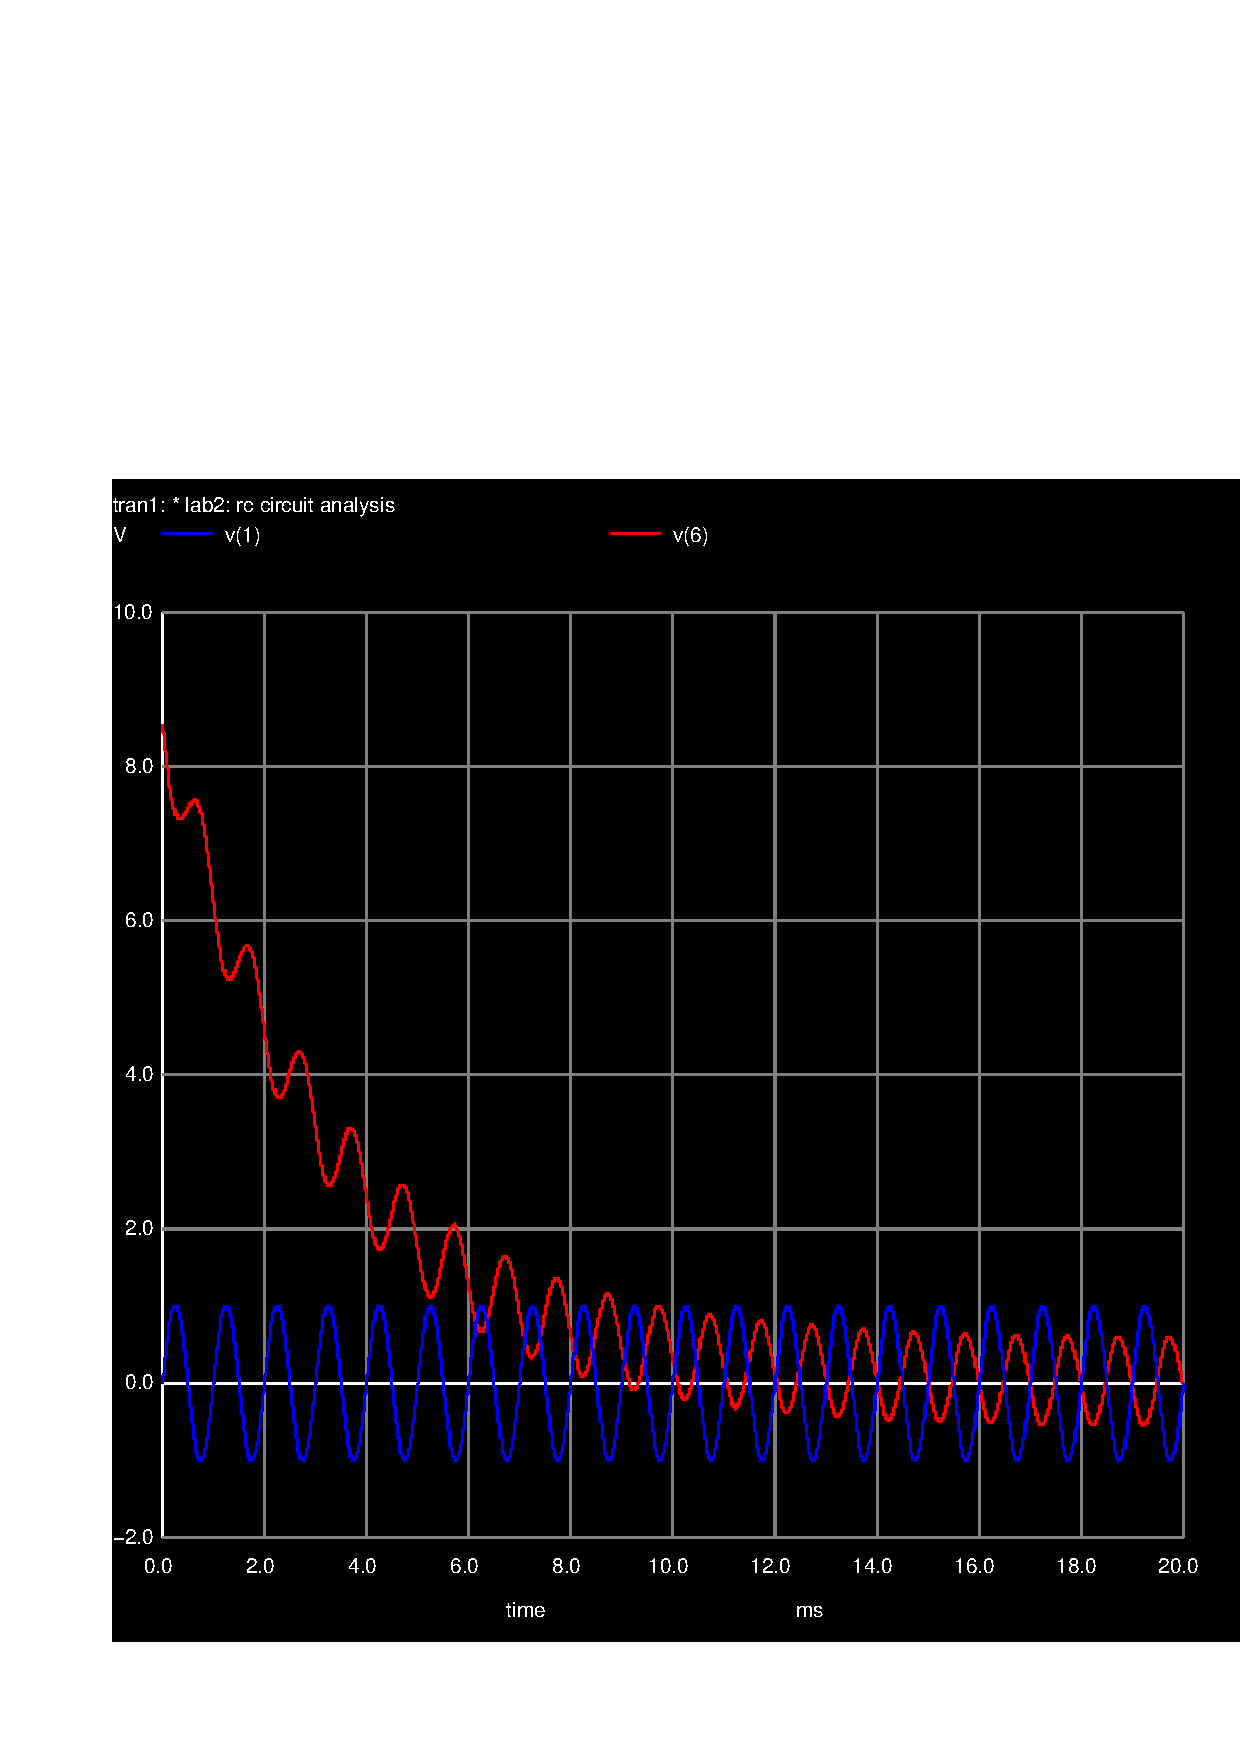
\includegraphics[scale = 0.55]{total.pdf}
         \caption{$v_{6}(t)$ and $v_{s}(t)$ in the interval $[0, 20]$ $ms$}
     \label{total}
 \end{figure}


\newpage
\subsection{Frequency analysis}

\vspace{5mm}
Using \textit{Ngpice}’s frequency analysis mode, the dependency of $v_s=v_1$, $v_6$ and $v_c$ on the frequency $f(Hz)$ of the input was studied. Figures \ref{acm} and \ref{acp} represent, respectively, the magnitude in $dB$ $db(v_1)$, $db(v_6)$ and $db(v_c)=db(v_6,v_8)$ and the phase in degrees $ph(v_1)$, $ph(v_6)$ and $ph(v_c)=ph(v_6,v_8)$ as a function of $f$. Note that it was chosen a logarithmic scale for the frequency axis (the space between each two consecutive vertical white lines represents a decade) and that both plots were made for a frequency range of $0.1$ $Hz$ to $1$ $MHz$.

 \begin{figure}[h]
     \centering
         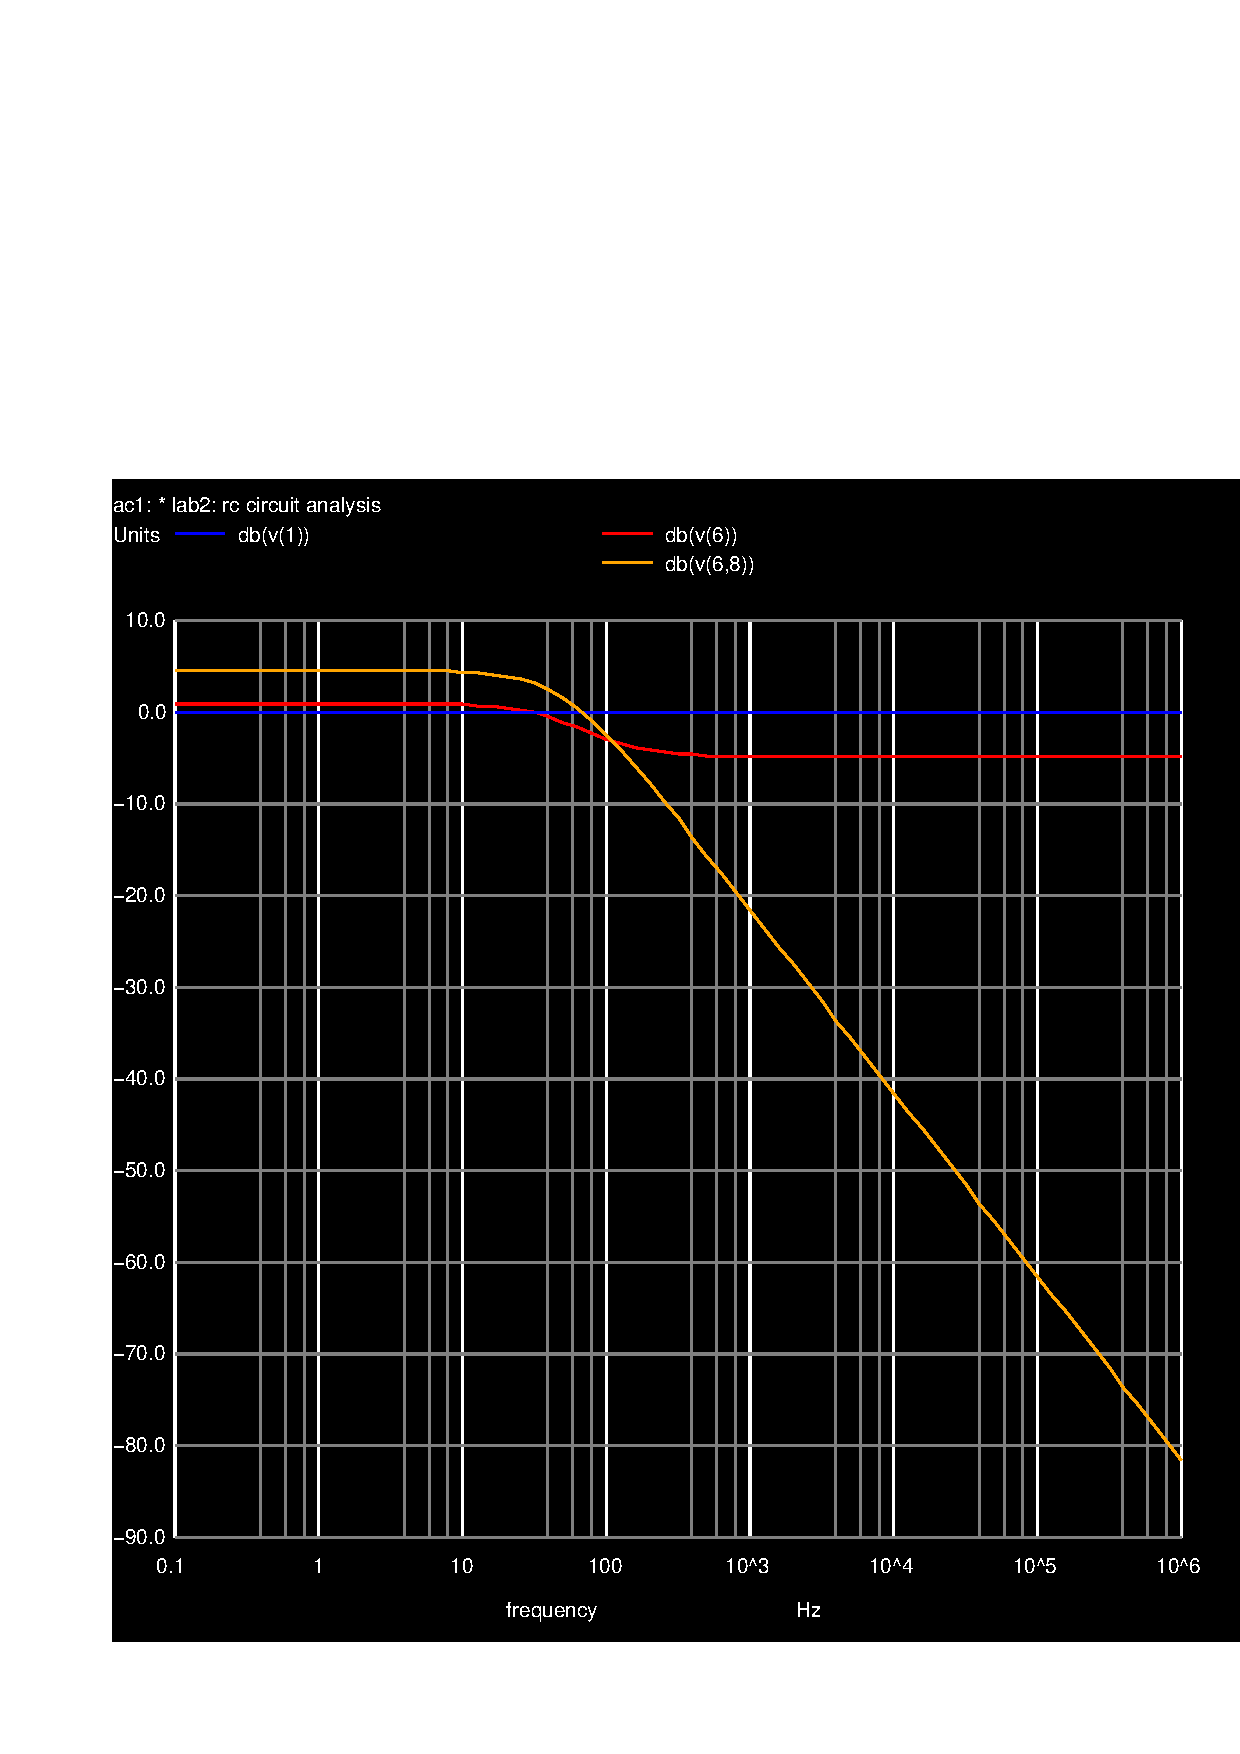
\includegraphics[scale = 0.55]{acm.pdf}
         \caption{Magnitude in $dB$ $db(v_1)$, $db(v_6)$ and $db(v_c)=db(v_6,v_8)$ as a function of $f$.}
     \label{acm}
 \end{figure}
 \vspace{5mm}

 \begin{figure}[h]
     \centering
         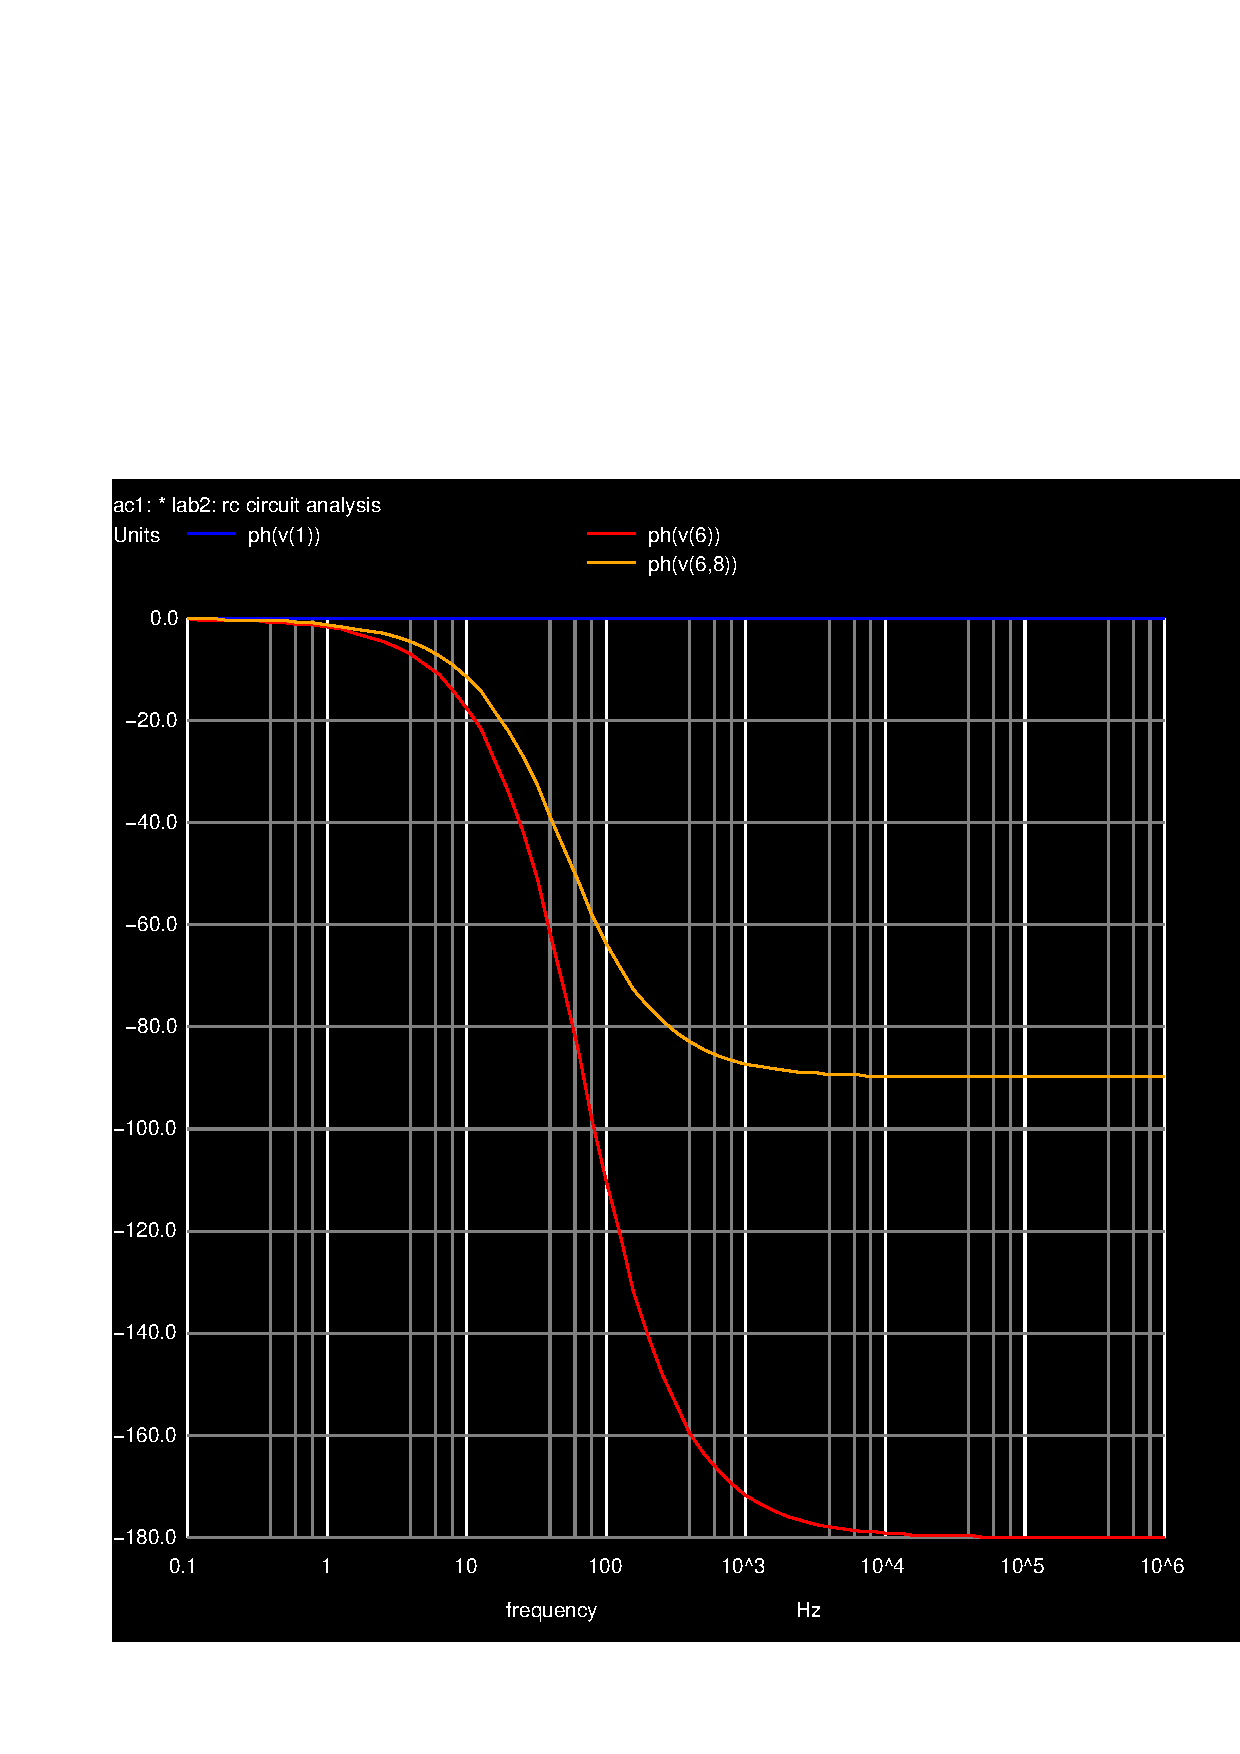
\includegraphics[scale = 0.55]{acp.pdf}
         \caption{Phase in degrees $ph(v_1)$, $ph(v_6)$ and $ph(v_c)=ph(v_6,v_8)$ as a function of $f$.}
     \label{acp}
 \end{figure}
 
\vspace{3mm}
\par Consult subsection \ref{teo:2.6} the conclusions related to the several plots (how and why the differ).

\newpage

